\chapter{Технологический раздел}\label{sec:impl}

\section{Средства реализации}

В качестве языка реализации был выбран Golang \cite{GO}, т\,к обладает достаточным набором необходимых инструментов для написания для написания веб-приложений: предоставляет базовый интерфейс маршрутизации, который в данной реализации был расширен с помощью пакета Gin \cite{GIN}, интерфейс работы с базами данных, а также имеет стандартные пакеты профилирования и тестирования \cite{testing}.

%Язык Golang[25] обладает достаточным набором инструментов для напи-
%сания одностраничных приложений: предоставляет базовые возможности
%маршрутизации, интерфейс работы с базами данных и конфигурационны-
%ми файлами, поэтому он был выбран в качестве реализации клиентского
%приложения. Базовый интерфейс маршрутизации был расширен с помо-
%щью пакета Gorilla[26].

\section{Реализация триггера}

Для спроектированных триггеров были написаны соответствующие функции с помощью PL/pgSQL \cite{PL}.

На листинге \ref{lst:get-age-category} представлена вспомогательная функция, которая определяет возрастную категорию, по дате рождения спортсмена.

\begin{figure}[H]
	\begin{lstlisting}[label=lst:get-age-category,caption=Реализация вспомогательной функции get\_age\_category() ]
create or replace function get_age_category(b date) 
returns varchar(10) as 
$$
begin 
	if (current_date - b) < 12 * 365 then 
		return 'children';
	end if;
	if (current_date - b) < 16 * 365 then
		return 'cadets';
	end if;
	if (current_date - b) < 23 * 365 then
		return 'juniors';
	end if;
	return 'adults';
	end;
$$ language plpgsql;
	\end{lstlisting}
\end{figure}

На листинге \ref{lst:trigger-insert} представлена функция триггера на добавление заявки на участие в турнире.

\begin{figure}[H]
\begin{lstlisting}[label=lst:trigger-insert,caption=Реализация триггера BEFORE на добавление заявки ]
create or replace function updateNum() returns trigger as $$
	declare 
		bd date;
	begin
		bd := (select birthday from account a where a.email = new.email);
		if (select sex 
			from account a 
			where a.email = new.email) = (select sex 
										  from competitions c 
										  where c.id = new.id_competition) 
			and (get_age_category(bd) = (select age_category 
										from competitions c 
										where c.id = new.id_competition)) 
			then 
				update competitions
				set numOfAthlets = (select numOfAthlets 
									from competitions 
									where id=new.id_competition) + 1
				where id=new.id_competition;
				return new;
		else
			raise exception 'You cannot apply for this tournament!';
		end if;
	end;
$$ language plpgsql;

create trigger updateNum before insert on AthletComp
for each row execute function updateNum();
\end{lstlisting}
\end{figure}

На листинге \ref{lst:trigger-del} представлена функция триггера на отмену заявки на участие в турнире.

\begin{figure}[H]
	\begin{lstlisting}[label=lst:trigger-del,caption=Реализация триггера AFTER на удаление заявки ]
create trigger decNum after delete on AthletComp
for each row execute function decNum();

create or replace function decNum() returns trigger as $$
	begin
		update competitions
		set numOfAthlets = (select numOfAthlets 
							from competitions 
							where id=old.id_competition) - 1
		where id=old.id_competition;
		return old;
	end
$$ language plpgsql;
	\end{lstlisting}
\end{figure}

\section{Сценарии выделения ролей}

На листинге \ref{lst:roles} представлены сценарии выделения ролей, спроектированных ранее.

\begin{figure}[H]
	\begin{lstlisting}[label=lst:roles,caption=сценарии выделения ролей]
grant select on table competitions to guest;
grant insert on table users to guest;

grant insert on table  athletcomp to use;
grant delete on table  athletcomp to use;
grant select on table  athletcomp to use;

grant insert on table  users to use;
grant select on table  competitions to use;
grant select on table  account to use;

create role administrator login password '1234';
grant all privileges on table users to administrator;
grant all privileges on table competitions to administrator;
grant all privileges on table battles to administrator;
grant all privileges on table athletcomp to administrator;
grant all privileges on table athlets to administrator;
	\end{lstlisting}
\end{figure}

\section{Реализация клиентского приложения}

%На листингах \ref{lst:account} - \ref{lst:battle} представлены модельные структуры для сущностей, представленных на рисунке \ref{ris:entity}.
%
%\begin{figure}[H]
%\begin{lstlisting}[label=lst:account,caption=Модельная структура сущности <<Аккаунт>>]
%type Account struct {
%	ID       int       `json:"id"`
%	Name     string    `json:"name"`
%	Birthday time.Time `json:"birthday"`
%	Sex      string    `json:"sex"`
%	Email    string    `json:"email"`
%}
%\end{lstlisting}
%\end{figure}
%
%\begin{figure}[H]
%\begin{lstlisting}[label=lst:ac,caption=Модельная структура сущности <<Заявка>>]
%type AthletComp struct {
%	ID     int    `json:"id"`
%	Email  string `json:"email"`
%	IDComp int    `json:"id_competition"`
%}
%\end{lstlisting}
%\end{figure}
%
%\begin{figure}[H]
%\begin{lstlisting}[label=lst:user,caption=Модельная структура сущности <<Пользователь>>]
%type User struct {
%	ID       int    `json:"id"`
%	Email    string `json:"email"`
%	Password string `json:"password"`
%	Role     string `json:"role"`
%	Verified bool
%}
%\end{lstlisting}
%\end{figure}
%
%\begin{figure}[H]
%\begin{lstlisting}[label=lst:battle,caption=Модельная структура сущности <<Бой>>]
%type Battle struct {
%	ID            int `json:"id"`
%	IDWinner      int `json:"id_winner"`
%	IDLooser    int `json:"id_looser"`
%	IDCompetition int `json:"id_competition"`
%	ScoreWinner   int `json:"score_winner"`
%	ScoreLooser int `json:"score_looser"`
%}
%\end{lstlisting}
%\end{figure}

База данных только хранит хешированный пароль. Функция регистрации пользователя, хеширование пароля и занесение его в базу данных представлены на листинге \ref{lst:sign-up}.

\begin{figure}[H]
	\begin{lstlisting}[label=lst:sign-up,caption=Функция регистрации пользователя]
func (a *AuthUseCase) SignUp(ctx context.Context, email,
							 password, role string) error {
	pwd := sha1.New()
	pwd.Write([]byte(password))
	pwd.Write([]byte(a.hashSalt))

	user := &models.User{
		Email:    email,
		Password: fmt.Sprintf("%x", pwd.Sum(nil)),
		Role:     role,
	}

	return a.userRepo.CreateUser(ctx, user)
}
	\end{lstlisting}
\end{figure}

Авторизация пользователя осуществляется через JWT \cite{JWT}. Функции авторизации и парсинга токена представлены на листингах \ref{lst:sign-in} и \ref{lst:parse} соответственно.

\begin{figure}[H]
	\begin{lstlisting}[label=lst:sign-in,caption=Функция авторизации пользователя]
func (a *AuthUseCase) SignIn(ctx context.Context, email, password, 
							 role string) (string, error) {
	pwd := sha1.New()
	pwd.Write([]byte(password))
	pwd.Write([]byte(a.hashSalt))
	password = fmt.Sprintf("%x", pwd.Sum(nil))

	user, err := a.userRepo.GetUser(ctx, email, password)
	if err != nil {
		return "", auth.ErrUserDoesNotExist
	}

	claims := AuthClaims{
	User: user,
	StandardClaims: jwt.StandardClaims{
		ExpiresAt: jwt.At(time.Now().Add(a.expireDuration)),
		},
	}

	token := jwt.NewWithClaims(jwt.SigningMethodHS256, claims)
	
	return token.SignedString(a.signingKey)
}
\end{lstlisting}
\end{figure}

\begin{figure}[H]
\begin{lstlisting}[label=lst:parse,caption=Функция парсинга токена]	
func (a *AuthUseCase) ParseToken(ctx context.Context, accessToken string) 
								(*models.User, error) {
	token, err := jwt.ParseWithClaims(accessToken, &AuthClaims{}, 
									  func(token jwt.Token) 
									  (interface{}, error) {
		if _, ok := token.Method.(*jwt.SigningMethodHMAC); !ok {
			return nil, 
				   fmt.Errorf("unexpected signing method: %v", 
				   token.Header["alg"])
		}
		return a.signingKey, nil
	})

	if err != nil {
		fmt.Println(err.Error())
		return nil, err
	}

	if claims, ok := token.Claims.(*AuthClaims); ok && token.Valid {
		return claims.User, nil
	}

	return nil, auth.ErrInvalidAccessToken
}
	\end{lstlisting}
\end{figure}

\section{Интерфейс приложения}

На данный момент доступен технический интерфейс, реализованный с помощью Postman \cite{Postman}.

На рисунке \ref{ris:sign-in} представлен пример успешной авторизации. В качестве ответа выдается JWT, который далее используется для доступа к другим эндпоинтам.

\begin{figure}[H]
	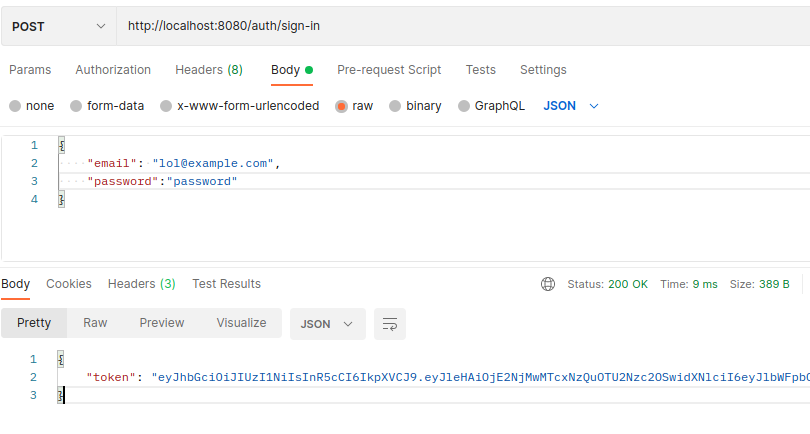
\includegraphics[width=1\columnwidth]{assets/signIn.png}
	\centering
	\caption{Пример успешной авторизации}
	\label{ris:sign-in}
\end{figure}

На рисунке \ref{ris:before} представлен пример запроса к эндпоинту /competition с параметром id = 1. На момент данного запроса еще никто не подал заявку на участие в данном турнире.

\begin{figure}[H]
	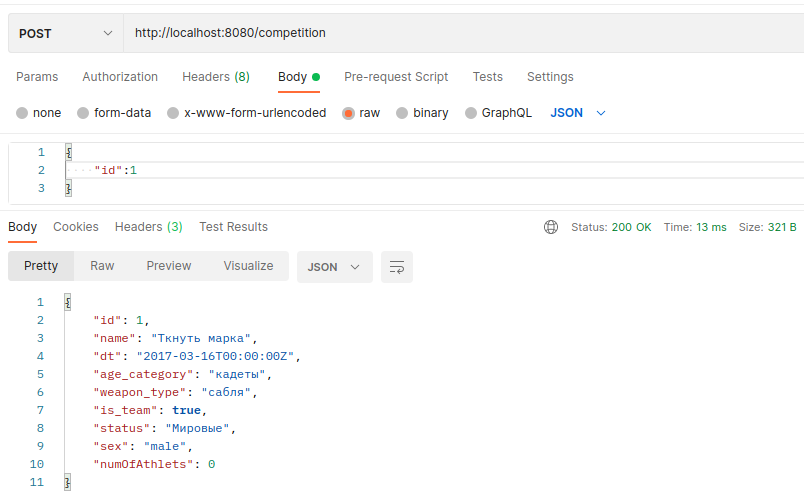
\includegraphics[width=1\columnwidth]{assets/before.png}
	\centering
	\caption{Запрос к эндпоинту /competition}
	\label{ris:before}
\end{figure}

На рисунке \ref{ris:newRequest} представлена успешная подача заявки на соревнование 1. 

\begin{figure}[H]
	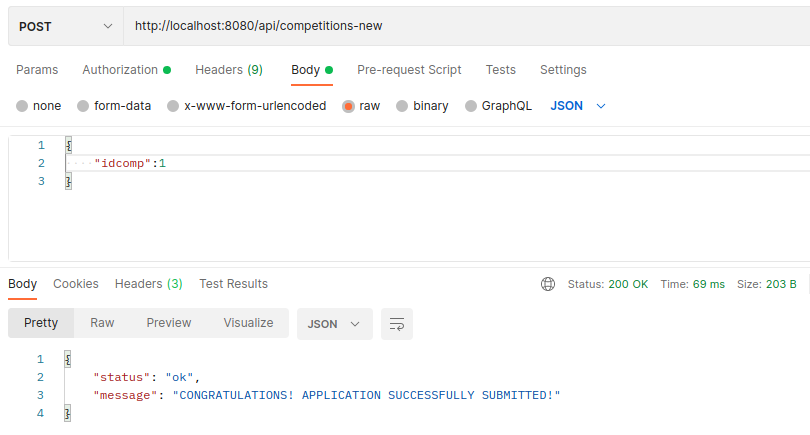
\includegraphics[width=1\columnwidth]{assets/newRequest.png}
	\centering
	\caption{Создание новой заявки на участие в соревновании}
	\label{ris:newRequest}
\end{figure}

На рисунке \ref{ris:before} представлен еще один пример запроса к эндпоинту /competition с параметром id = 1. Стоит отметить, что после подачи заявки число участников соревнований увеличилось.

\begin{figure}[H]
	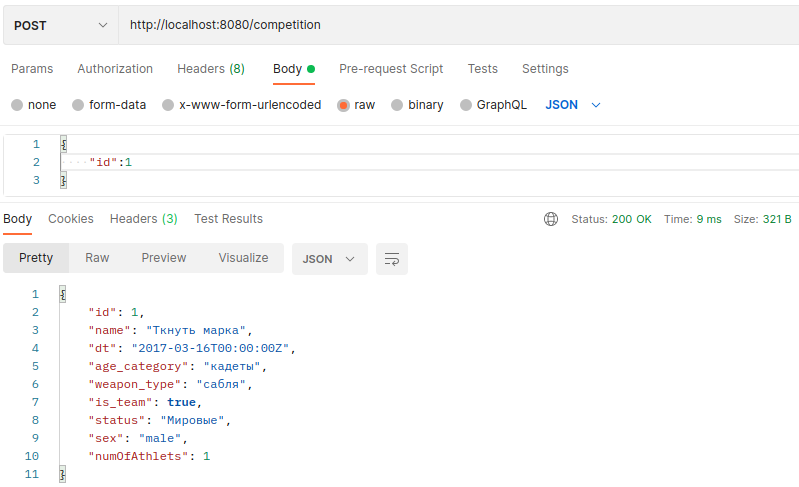
\includegraphics[width=1\columnwidth]{assets/after.png}
	\centering
	\caption{Запрос к эндпоинту /competition}
	\label{ris:after}
\end{figure}

На рисунке \ref{ris:delRequest} представлен пример отмены заявки на участие в турнире 1.

\begin{figure}[H]
	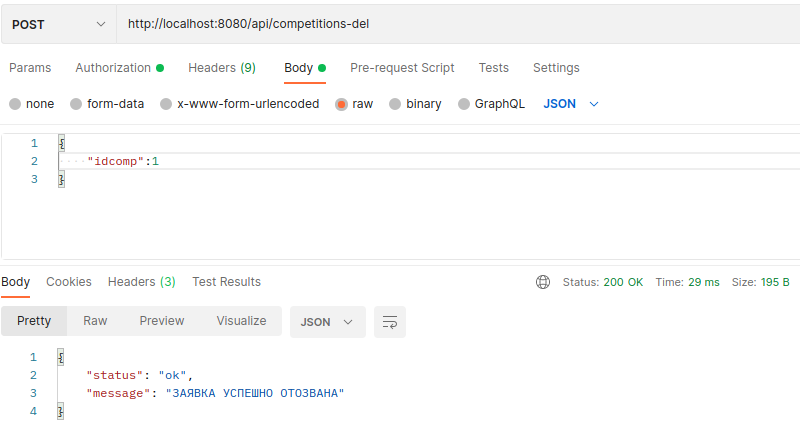
\includegraphics[width=1\columnwidth]{assets/delRequest.png}
	\centering
	\caption{Отмена заявки на участие в соревновании}
	\label{ris:delRequest}
\end{figure}

Как можно заметить на рисунке \ref{ris:final} число участников после отмены заявки на участие уменьшилось.

\begin{figure}[H]
	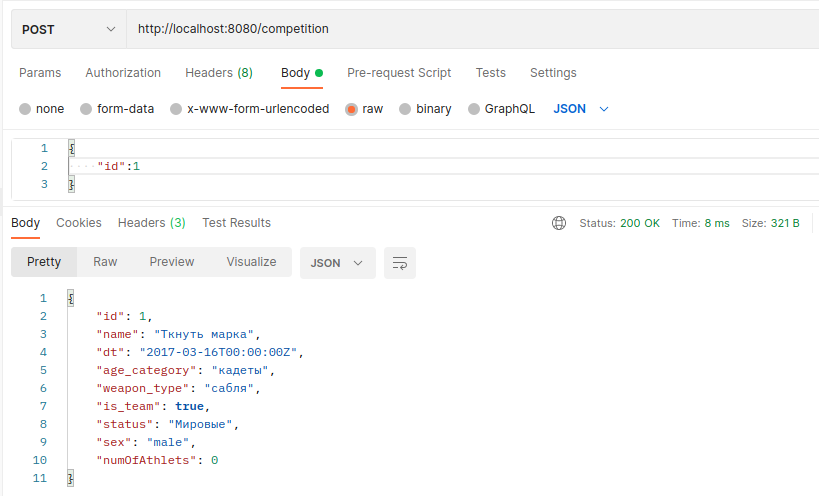
\includegraphics[width=1\columnwidth]{assets/final.png}
	\centering
	\caption{Запрос к эндпоинту /competition}
	\label{ris:final}
\end{figure}

\section{Заполнение базы данных}

Для заполнения базы данных были специально написаны скрипты на языке программирования Python \cite{python} с помощью библиотеки Mimesis \cite{mimesis}, позволяющей генерировать фейковые данные.

Основные функции для заполнения таблицы competitions приведены на листинге \ref{lst:python}.

\begin{figure}[H]
	\begin{lstlisting}[label=lst:python,caption=функции для генерация данных для таблицы competitions]
def randomAgeCategory():
	data = ['children', 'cadets', 'juniors', 'adults']
return choice(data)

def randomWeaponType():
	data = ['foil', 'saber', 'epee']
return choice(data)

def randomStatus():
	data = ['World', 'European', 'Russian']
return choice(data)

def randomSex():
	data = ['female', 'male']
return choice(data)

def competitionDescription():
	f = Field('ru')
	return {
		'name': ' '.join(f('words', quantity=2)).capitalize(),
		'dt': f('date'),
		'age_category': randomAgeCategory(),
		'weapon_type': randomWeaponType(),
		'is_team': f('boolean'),
		'status': randomStatus(),
		'sex': randomSex(),
		'count': 0
	}
	\end{lstlisting}
\end{figure}

\section{Вывод}

В данном разделе были описаны средства реализации, основные реализованные функции, представлены сценарии выделения ролей на уровне базы данных и приведены примеры работы приложения.